%\newpage

\section{Problem Definition}
\label{sec:problem-definition}
%\guy{Can someone check Sections 3-4-5? Especially the formulations}


\subsection{Background}
\label{subsec:background}

\textbf{Petri Nets.} 
A Petri net is $N=(P,T,\mathsf{pre},\mathsf{post},M_0)$ with places $P$, transitions $T$, input/output maps $\mathsf{pre},\mathsf{post}:T\to\mathbb N^P$, and initial marking (token distribution) $M_0\in\mathbb N^P$.  
A transition $t$ is \textit{enabled} at marking $M \in \mathbb N^P$ if $M\ge \mathsf{pre}(t)$ coordinate-wise, i.e., $M$ provides at least as many tokens as required by $\mathsf{pre}(t)$.
%
If an enabled transition \(t\) \textit{fires} (denoted $M\xrightarrow{t}M'$), it produces the marking $M' = M - \mathsf{pre}(t) + \mathsf{post}(t)$ consuming input tokens and producing output tokens.
%
This can extend naturally to a sequence of firings $\sigma = t_1\cdots t_k$ (denoted $M \xrightarrow{\sigma} M'$), giving rise to a sequence of markings $M_0,\ldots,M_k$ with $M=M_0$, $M'=M_k$, and $M_i \xrightarrow{t_{i+1}} M_{i+1}$ for all $i$. 
% 
We define the reachable set $R(N)=\{M \mid \exists \sigma\in T^*. M_0 \xrightarrow{\sigma} M\}$ to include all markings reachable from the initial state $M_0$.
% 
The \textit{reachability problem} asks, given a Petri net $N$ and a marking $M$, whether $M\in R(N)$. 
%
Specifically, we focus on reachability of a formula $F$, encoding a combination of linear constraints; it is \sat\ if some $M\in R(N)$ satisfies $F$ (marked $M \models F$), and otherwise \unsat{} (see the toy example in 	Appendix~\ref{appendix:toyPN}).
%
Surprisingly, even for the \textit{unbounded} setting, where places can hold unbounded many tokens, this problem is decidable~\cite{Ma81,Ko82,La92}, although Ackermann-complete~\cite{CzWo22,Le22}.   



\medskip
\noindent
\textbf{Verdict proofs.} 
If $F$ is reachable, a witness $\sigma\in T^*$ with $M_0\xrightarrow{\sigma}M$ and $M\models F$ is a proof, verifiable by simulation of the Petri net.  
If $F$ is unreachable, there exists~\cite{Le09} an inductive Presburger certificate $C$ such that:  
(i) $M_0\models C$, (ii) $M\models C \wedge M\xrightarrow{t}M'\Rightarrow M'\models C$, and (iii) $C\Rightarrow \neg F$.

\medskip
\noindent
\textbf{Semilinear sets and Parikh’s theorem.} 
A set $S\subseteq\mathbb N^k$ is \textit{semilinear} iff  
$S=\bigcup_{i=1}^m \{\mathbf b_i+\sum_{j=1}^{r_i} n_j\mathbf p_{i,j}\mid n_j\in\mathbb N\}$,  
for $\mathbf b_i,\mathbf p_{i,j}\in\mathbb N^k$.  
Semilinear sets coincide with sets defined by \textit{Presburger arithmetic}~\cite{Pr29}.  
By Parikh’s theorem~\cite{Parikh66}, the \textit{Parikh Image} of any context-free language is semilinear, with an effective construction.

\medskip
\noindent
\textbf{Deciding serializability in unbounded systems.} 
Bouajjani et al.~\cite{BoEmEnHa13} have proved that serializability in unbounded systems reduces to Petri net reachability, as a special case of \textit{bounded-barrier linearizability}.


\subsection{The SER Language}
%\subsection{Syntax}
Our \toolname{} syntax is defined as follows: 
%of Fig.~\ref{fig:syntax}.

\[
\begin{aligned}
	\mathbf{Expression}\quad e ::= &\ 0 \mid 1 \mid 2 \mid \dots            && \text{numeric const.}\\
	&\mid \nondet                            && \text{nondet.\ value (0/1)}\\
	&\mid x := e \mid x                      && \text{write/read local var}\\
	&\mid X := e \mid X                      && \text{write/read global var}\\
	&\mid e_1 == e_2                         && \text{equality test}\\
	&\mid e_1 ; e_2                          && \text{sequencing}\\
	&\mid \ifkw(e_1)\{e_2\}\elsekw\{e_3\}    && \text{conditional}\\
	&\mid \whilekw(e_1)\{e_2\}               && \text{while loop}\\
	&\mid \yieldkw                           && \text{yield to scheduler}
	\\[0.8em]
	\mathbf{Program}\quad p ::= &\ \requestkw\ name_1\{e_1\}\;\dots\;\requestkw\ name_n\{e_n\}
	&& \text{set of request handlers}
\end{aligned}
\]

%
%\[
%\begin{aligned}
%	\mathbf{Expression}\quad e ::={}&{} \\
%	&0 \mid 1 \mid 2 \mid \dots 
%	&&\grammartag{Numeric constants}\\
%	&\nondet
%	&&\grammartag{Nondeterministic value: 0 or 1}\\
%	&x := e
%	&&\grammartag{Write to local variable}\\
%	&x
%	&&\grammartag{Read from local variable}\\
%	&X := e
%	&&\grammartag{Write to global variable}\\
%	&X
%	&&\grammartag{Read from global variable}\\
%	&e_1 == e_2
%	&&\grammartag{Equality test}\\
%	&e_1 ; e_2
%	&&\grammartag{Sequencing}\\
%	&\ifkw(e_1)\{e_2\}\elsekw\{e_3\}
%	&&\grammartag{Conditional}\\
%	&\whilekw(e_1)\{e_2\}
%	&&\grammartag{While loop}\\
%	&\yieldkw
%	&&\grammartag{Yields to scheduler}\\[1em]
%	\mathbf{Program}\quad p ::={}&{} \\
%	&\requestkw\ name_1\{e_1\}
%	&&\grammartag{Set of request handlers}\\
%	&\quad\vdots\\
%	&\requestkw\ name_n\{e_n\}
%\end{aligned}
%\]
%
%%
%
%\begin{figure}[!htbp]
%    \begin{align*}
%    \mathbf{Expression}\quad e ::= &&& \\
%       | & \quad 0 \mid 1 \mid 2 \mid \ldots                                && \grammartag{Numeric constants} \\
%       | & \quad \nondet                                 && \grammartag{Nondeterministic value: 0 or 1}\\
%       | & \quad x := e                            && \grammartag{Write to local variable field} \\
%       | & \quad x                                 && \grammartag{Read from local variable field} \\
%       | & \quad X := e                            && \grammartag{Write to global  variable} \\
%       | & \quad X                                 && \grammartag{Read from global  variable} \\
%       | & \quad e_1 == e_2                        && \grammartag{Equality test} \\
%       | & \quad e_1 ; e_2                         && \grammartag{Sequencing} \\
%       | & \quad \ifkw(e_1)\{\ e_2\ \}\elsekw\{\ e_3\ \} && \grammartag{Conditional} \\
%       | & \quad \whilekw(e_1)\{\ e_2\ \}              && \grammartag{While loop} \\
%       | & \quad \yieldkw                      && \grammartag{Yields to scheduler}\\[1em]
%    \mathbf{Program}\quad p ::=
%        & \quad \requestkw\ name_1\ \{\ e_1\ \}&&\grammartag{Set of request handlers}\\[-0.5em]
%        & \quad \qquad \vdots &&\\
%        & \quad \requestkw\ name_n\ \{\ e_n\ \}\ 
%    \end{align*}
%    \caption{Syntax of expressians and programs}
%    \label{fig:syntax}
%\end{figure}
    %
%    
%
%
%
%\guy{add other rebuttal promises}
%\guy{check semantics}
%
%
% SER small-step semantics with explicit guard (congruence) rules
% Requires: \usepackage{mathtools,amssymb,mathpartir}



Our semantics is straightforward, and fully formalized in Appendix~\ref{appendix:ser-semantics}.
%
Furthermore, we note that our syntax and semantics can both be extended to include \textit{arithmetic operations} however, we omit these for simplicity. 
    
    
\subsection{Network System}    
We now present our abstract network system (NS) setting, which is motivated by software-defined networking. In the networking domain, spawning a request corresponds to sending a \textit{packet}, with each local variable mapped to a unique \textit{packet header field}; global variables correspond to variables on \textit{programmable switches}, as they are shared among all requests visiting the switch. Throughout this paper, we use the term \emph{request} to refer to a concurrent computation unit. 
%
We define a network system $\mathcal{N}$ as a tuple $(G, L, \mathit{REQ},  \mathit{RESP}, g_0, \delta, \mathit{req}, \mathit{resp})$ where:
\begin{itemize}
\item $G$ is a set of \textit{global network states} (e.g., a state variable on a switch)

\item $L$ is a set of \textit{local packet states} (e.g., a packet header value)

\item $\mathit{REQ}$ is a finite set of\textit{ request strings} (each marked {\color{ForestGreen}$\blacklozenge_\text{req}$})

\item $\mathit{RESP}$ is a finite set of \textit{response strings} (each marked {\color{red}$\blacklozenge_\text{resp}$})

\item $g_0 \in G$ is the \textit{initial global state} of the network system

\item $\mathit{req} \subseteq \mathit{REQ} \times  L$ maps each request to its corresponding local state --- this represents externally spawning a packet matching the request type

\item $\mathit{resp} \subseteq L \times \mathit{RESP}$ maps a final local state to the corresponding response (this represents a packet exiting the network and returning the computation)

\item $\delta \subseteq  (L \times G) \times ( L \times G)$ defines atomic execution steps that update both global and local state (this represents a packet doing a single hop in the network)
%(and the corresponding SER expressions); as based on SER's small-step semantics
\end{itemize}

%\todo{new start}
%We refer to our transition rules in Fig.~\ref{fig:code2ExampleNS}.

\smallskip
\noindent
\textbf{Request and response.}
A \emph{request} ${\color{ForestGreen}\blacklozenge_\text{r}} \in \mathit{REQ}$ represents the initiation of a concurrent computation unit. Each request has an associated handler expression from the program syntax that defines its behavior.
A \emph{response} ${\color{red}\blacklozenge_\text{s}} \in \mathit{RESP}$ represents the value returned by a request after its execution terminates.
The pair $({\color{ForestGreen}\blacklozenge_\text{r}}, {\color{red}\blacklozenge_\text{s}}) \in \mathit{REQ} \times \mathit{RESP}$ captures the complete input-output behavior of a single request execution.


\smallskip
\noindent
\textbf{States.}
A (global) \emph{network state} is a triple $(g,\mathcal{P},Z)$ where
$g \in G$ is the current global network state,
$\mathcal{P} \in \mathrm{Multiset}(L \times \mathit{REQ})$ is a multiset of in-flight requests (threads, i.e., triplets of SER expressions, local thread states, and the original request strings),
and $Z \in \mathrm{Multiset}(\mathit{REQ} \times \mathit{RESP})$ is a multiset of completed request/response pairs.
%
The initial global state is $(g_0, \varnothing, \varnothing)$.




% Non-figure version of the state-transition rules (caption text inlined)
%\renewcommand{\arraystretch}{1.6}
%\medskip
\smallskip
\noindent
\textbf{Transition rules.}
A transition \(\longrightarrow\) modifies the triple \((g,\mathcal{P}, Z)\) by either
(1) introducing a new request, (2) processing a request step via \(\delta\), or
(3) consuming a request to produce its response. When no more steps are possible,
the result set \(Z\) is the final multiset of request/response pairs that arose during the run.



%\noindent\textbf{States and transitions.}
%A (global) \emph{network state} is a triple $(g,\mathcal{P},M)$ where
%$g \in G$ is the current global state,
%$\mathcal{P} \in \mathrm{Multiset}(L \times \mathit{REQ})$ is a multiset of in-flight requests (threads),
%and $M \in \mathrm{Multiset}(\mathit{REQ} \times \mathit{RESP})$ is a multiset of completed request/response pairs.
%%
%The initial state is $(g_0, \varnothing, \varnothing)$.


%\smallskip
%\noindent\textbf{Initial state.} $(g_0, \varnothing, \varnothing)$.

%\smallskip
%\noindent\textbf{Transition rules.}
\[
\text{(New Request)}\quad
\infer{({\color{ForestGreen}\blacklozenge_\text{r}},\ell)\in\mathit{req}}
{(g,\mathcal{P},Z) \rightarrow (g,\; \mathcal{P}\uplus\{(\ell,{\color{ForestGreen}\blacklozenge_\text{r}})\},\; Z)}
\]
\[
\text{(Processing Step)}\quad
\infer{((\ell, g),(\ell', g'))\in\delta}
{(g,\; \mathcal{P}\uplus\{(\ell,{\color{ForestGreen}\blacklozenge_\text{r}})\},\; Z)
	\rightarrow
	(g',\; \mathcal{P}\uplus\{(\ell',{\color{ForestGreen}\blacklozenge_\text{r}})\},\; Z)}
\]
\[
\text{(Response)}\quad
\infer{(\ell,{\color{red}\blacklozenge_\text{s}})\in\mathit{resp}}
{(g,\; \mathcal{P}\uplus\{(\ell,{\color{ForestGreen}\blacklozenge_\text{r}})\},\; Z)
	\rightarrow
	(g,\; \mathcal{P},\; Z \uplus \{({\color{ForestGreen}\blacklozenge_\text{r}},{\color{red}\blacklozenge_\text{s}})\})}
\]


\smallskip
\noindent
\textbf{Serializability.}
An \textit{interleaving run} is a complete execution 
\((g_0,\varnothing,\varnothing)\!\to^*\!(g_n,\varnothing,Z)\):
\[
(g_0,\varnothing,\varnothing) \;\to\; (g_1,\mathcal{P}_1,Z_1) \;\to\; \cdots \;\to\; (g_{n-1},\mathcal{P}_{n-1},Z_{n-1}) \;\to\; (g_n,\varnothing,Z).
\]
It is said to be \textit{serial} if each $\mathcal{P}_i$ has \textit{at most} one request, and $\mathcal{P}_n=\varnothing$.
	%
	Intuitively, serial runs have at most one request in flight at any time.
%	,
%	whereas \emph{interleaved} runs may have multiple requests in flight at once.
	%
	
	For a network system \(\mathcal{N}\), we define \(\mathrm{Int}(\mathcal{N})\) and \(\mathrm{Ser}(\mathcal{N})\) to respectively represent the sets of all multisets of request/response pairs, for interleaving and serializable runs :
%
\[
\mathrm{Int}(\mathcal{N})
= \bigl\{\, Z \in \mathrm{Multiset}(\mathit{REQ}\times \mathit{RESP})
\;\big|\; \exists\ \text{\textit{interleaved} run } (g_0,\varnothing,\varnothing)\rightarrow^{*}(g_n,\varnothing,Z) \,\bigr\}
\]
%
\[
\mathrm{Ser}(\mathcal{N})
= \bigl\{\, Z \in \mathrm{Multiset}(\mathit{REQ}\times \mathit{RESP})
\;\big|\; \exists\ \text{\textit{serial} run } (g_0,\varnothing,\varnothing)\rightarrow^{*}(g_n,\varnothing,Z) \,\bigr\}.
\]

A network system is \emph{serializable} if \(\mathrm{Int}(\mathcal{N})=\mathrm{Ser}(\mathcal{N})\), i.e., every multiset of request/response pairs attained by an interleaving execution can also be attained serially.


%
%\todo{old}
%\smallskip
%\noindent
%\textbf{Serializability.}
%We define an \textit{interleaving run} of the network system as a complete execution (also denoted \((g_0,\varnothing,\varnothing)\rightarrow^{*}(g_n,\varnothing,Z)\)):
%%\noindent\textbf{Complete runs.}
%\[
%(g_0,\varnothing,\varnothing) \rightarrow (g_1,\mathcal{P}_1,Z_1)
%\rightarrow \cdots \rightarrow (g_n,\mathcal{P}_{n-1},Z_{n-1}) \rightarrow (g_n,\varnothing,Z_n).
%\]
%
%\noindent
%%A full run is also denoted \((g_0,\varnothing,\varnothing)\rightarrow^{*}(g_n,\varnothing,Z)\), and is called an \textit{interleaved} run if the $\mathcal{P}_i$ may contain multiple requests and $\mathcal{P}_n=\varnothing$.
%%
%An interleaved run is said to be \textit{serial} if each $\mathcal{P}_i$ has \textit{at most} one request, and $\mathcal{P}_n=\varnothing$.
%%
%Intuitively, \textit{serial} runs have at most one request in flight at any time,
%whereas \emph{interleaved} runs may have multiple requests in flight at once.
%%
%For a network system \(\mathcal{N}\), we define \(\mathrm{Int}(\mathcal{N})\) and \(\mathrm{Ser}(\mathcal{N})\) to  represent the set of all multisets of request/response pairs, for interleaving and serializable runs respectively:
%
%\[
%\mathrm{Int}(\mathcal{N})
%= \bigl\{\, Z \in \mathrm{Multiset}(\mathit{REQ}\times \mathit{RESP})
%\;\big|\; \exists\ \text{\textit{interleaved} run } (g_0,\varnothing,\varnothing)\rightarrow^{*}(g_n,\varnothing,Z) \,\bigr\}
%\]
%\[
%\mathrm{Ser}(\mathcal{N})
%= \bigl\{\, Z \in \mathrm{Multiset}(\mathit{REQ}\times \mathit{RESP})
%\;\big|\; \exists\ \text{\textit{serial} run } (g_0,\varnothing,\varnothing)\rightarrow^{*}(g_n,\varnothing,Z) \,\bigr\}.
%\]
%
%
%
%A network system $\mathcal{N}$ is \emph{serializable} if $\text{Int}(\mathcal{N}) = \text{Ser}(\mathcal{N})$, i.e., every multiset of request/response pairs attainable through an interleaved execution can also be attained through a serial one.

\subsection{Translating \toolname{} programs to NS}
%
The NS abstraction is useful beyond its capability to capture concurrent behaviors in software-defined networks.
%
Specifically, another advantage is the natural translation from  \toolname{} programs to their corresponding NS.
%, as we demonstrate next.
%
%
%\smallskip
%\noindent
Given a \toolname{} program \(P_0\) with: (i) an initial local state \(\rho_0\); (ii) an initial global state \(g_0\); (iii) local variables (\(vars\)); (iv) global variables (\(VARS\)); (v) mappings \(\rho\) and (vi) \(g\) from local/global variables to (vii) a finite set of values \(V\), we define the following NS $(G, L, \mathit{REQ},  \mathit{RESP}, g_0, \delta, \mathit{req}, \mathit{resp})$:

\[
\begin{aligned}
	G \;&=\; \{\, g : \text{VARS}\!\to\! V \,\},\\[0.3ex]
	L \;&=\; \bigl\{\, (e,\rho)\ \bigm|\ \rho:\text{vars}\!\to\! V,\ \exists\,name_i\{e_i\}\!\in\! P_0,\ \exists k\!\ge\!0\ \text{s.t.} \\[-0.2ex]
	&\qquad\quad\qquad\quad e \text{ is the suffix of } e_i \text{ up to the next } \yieldkw \text{ or termination} \,\bigr\},\\[0.3ex]
	REQ \;&=\; \{\, name_i \mid name_i\{e_i\}\!\in\! P_0 \,\},\quad RESP \;=\; V,\\[0.3ex]
	req \;&=\; \{\, (r,\ell) \mid r=name_i\!\in\!REQ,\ \ell=(e_i,\rho_0)\!\in\!L \,\},\\[0.3ex]
	resp \;&=\; \{\, (\ell',r') \mid \exists v\!\in\!V.\ \ell'=(v,\rho')\!\in\!L,\ r'=v\!\in\!RESP \,\},\\[0.3ex]
	\delta \;&=\; \bigl\{\, ((e,\rho),g)\!\to\!((e',\rho'),g') \ \bigm|\ (e,\rho),(e',\rho')\!\in\!L,\ g,g'\!\in\!G,\ 
	\cfg{e}{\rho}{g} \pstep \cfg{v}{\rho'}{g'} \,\bigr\}.
\end{aligned}
\]


%
%\begin{itemize}
%	\item The set of global states include all mappings from global variables to values:
%	\[
%	G = \{\, g \mid g : \text{VARS} \to V \,\}.
%	\]
%	
%	\item The set of local states include a pair of the local variable assignments coupled with the remaining \toolname{} program to execute, i.e., a sequence of expressions until: (i) the subsequent \(\yieldkw\); or (ii) termination
%	\[
%	L = \{\, (r,\rho) \mid \exists \rho : \text{vars} \to V \ \exists \, name_i\{e_i\} \in P_0 \ \exists k \ge 0 \,.\, (e_k';\yieldkw)^k ; e = e_i \in P_0 \,\}.
%	\]
%
%	
%	\item The set of requests are the handlers of the \toolname{} program:
%	\[
%	REQ = \{\, name_i \mid name_i\{e_i\} \in P_0 \,\}.
%	\]
%	
%	\item The set of responses include all possible numerical constants:
%	\[
%	RESP = V.
%	\]
%	
%	\item The request relation maps every request to a local state with the corresponding request handler and the initial local assignment:
%	\[
%	req = \{\, (r,\ell) \mid r = name_i \in REQ, \, \ell = (e_i,\rho_0) \in L \,\}.
%	\]
%	
%	\item The response relation maps the computed constant (attained prior to termination) with the corresponding response:
%	\[
%	resp = \{\, (\ell',r') \mid \exists v \in V \,.\, \ell' = (v',\rho') \in L, \, r' \in RESP \,\}.
%	\]
%	
%	\item The transition relation, defined according to the \toolname{} semantics:
%	\[
%	\delta = \bigl\{ \, 
%	(((e,\rho),g),((e',\rho'),g')) \,\bigm|\, 
%	(e,\rho),(e',\rho') \in L, \ g,g' \in G, \ 
%	\cfg{e}{\rho}{g} \pstep \cfg{v}{\rho'}{g'} 
%	\,\bigr\}.
%	\]
%\end{itemize}
%



% $\mathit{req} \subseteq \mathit{REQ} \times  L$ maps each request type to its corresponding local state
%initial SER expression and  local state
%
% $\mathit{resp} \subseteq L \times \mathit{RESP}$ maps final SER expressions and local states to response types
%
% $\delta \subseteq  (L \times G) \times ( L \times G)$ defines atomic execution steps that update both global and local state 
%(and the corresponding SER expressions); as based on SER's small-step semantics



%\smallskip
%\noindent
%\textbf{Assumptions.}
%%
%In addition to the assumption that the request and response sets are finite, we also assume that a program has a \textit{finite number of reachable states}. 
%%
%These states are enumerated when converting a \toolname{} program to a Network System. 
%%
%For convenience, the input program may be written with unbounded values as long as only a finite number are actually reached. 
%%
%If the program can reach an infinite number of states, then this initial Network System conversion times out. 
%
%If the input program is written with restricted syntax shown in the SER syntax, then the SER \(\step\) NS conversion always terminates. 


%\subsection{NS Example: Non-Serializability }
%\label{sec:ns-non-serializable}
%\medskip
%\noindent
%\textbf{Example: \toolname{} to NS.}
%
\begin{tcolorbox}[colback=black!5!white, colframe=black, boxrule=1pt]
\textbf{Example.}
Recall the code snippet from the simple, non-serializable example presented in Listing~\ref{lst:MotivatingExample2NonSer}. We can represent its NS with the following mapping:

\begin{itemize}
\item 
The set $G$ is defined as $G=\{[\texttt{X=0}], [\texttt{X=1}]\}$.

\item 
The initial global state is defined as $g_0 = [\texttt{X=0}]$.

\item 
We define $L$ as all pairs of local states (assignments such as $[\texttt{y=0}], [\texttt{y=1}]$), coupled with all reachable \toolname{} programs (continuations of a program at a point of execution).
%~\footnote{
%These are continuations of a \toolname{} program at a point of execution. Concretely, this can mean either (i) the suffix of the program when it is first initialized (the part that has not yet executed); or (ii) the continuation of the program after a \(\yieldkw\) statement, where execution may later resume.}.
For example, the reachable programs for Listing~\ref{lst:MotivatingExample2NonSer} are depicted in Fig.~\ref{fig:code2ExampleNS}. 


\item 
The set of requests is $REQ = \{{\color{ForestGreen}\blacklozenge_\text{main}}\}$.

\item 
The set of responses is $RESP = \{{\color{red}\blacklozenge_0},{\color{red}\blacklozenge_1}\}$.

\item
The function \(\delta\) is presented in the bottom part of Fig.~\ref{fig:code2ExampleNS}.


\end{itemize}


We depict in Fig.~\ref{fig:code2ExampleNS} the explicit network system that
serves as a mapping from requests ({\color{ForestGreen}$\blacklozenge_\text{main}$}) to responses ({\color{red}$\blacklozenge_0$}, {\color{red}$\blacklozenge_1$}).
%
We note that we depicted only part of the states that are \textit{reachable}, in our finite-state setting.
%
\end{tcolorbox}

\begin{figure}[!htbp]
	\centering
	%–––– Network system diagram ––––
	% 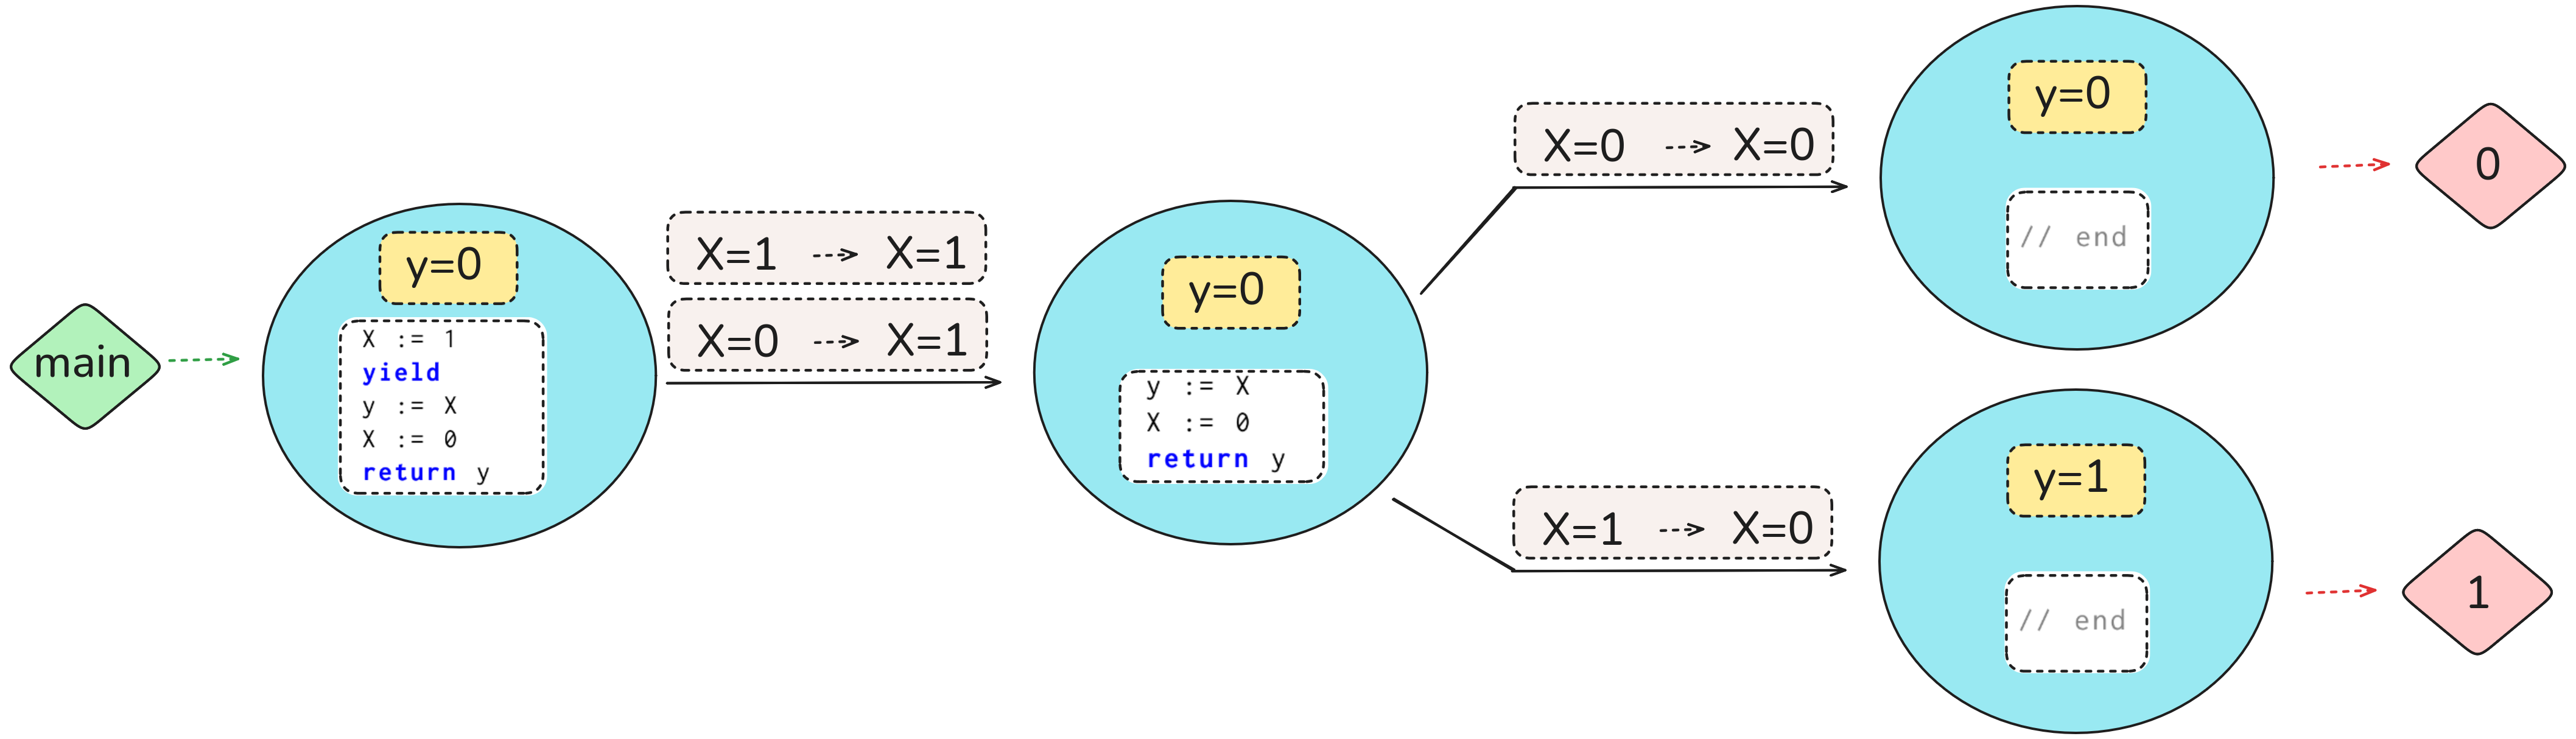
\includegraphics[width=\textwidth]{plots/code_2_NS.png}\\[1ex]

	\begin{tikzpicture}[
		node distance=1.5cm and 2.5cm,
		>=stealth,
		thick,
		every node/.style={font=\small}
	]
	  % [main request] -> [y=0][full program below that] ---[X=1 -> X=1][X=0 -> X=1 below that]--->[y=0][rest of program below that]
	  %   (first outgoing edge of last node on previous line)
      %   --[X=0 -> X=0]-->[y=0][empty program below that] ---> [0 response]
	  %   (second outgoing edge)
	  %   --[X=1 -> X=0]-->[y=1][empty program below that] ---> [1 response]
	  
	  % Main request node
	  \node[
		draw=black,
		line width=0.8pt,
		fill=ForestGreen!20,
		text=black,
		diamond,
		aspect=2,
		inner sep=2pt,
		scale=0.7
	  ] (main) {\texttt{main}};
	  
	  % First state node with full program
	  \node[right=0.7cm of main, align=center] (state1) {
		\begin{tikzpicture}[baseline=(ybox.base)]
			\node[
			draw=black,
			line width=0.8pt,
			fill=brightyellow,
			text=black,
			rectangle,
			rounded corners=1pt,
			inner sep=2pt
			] (ybox) {\texttt{y=0}};
		\end{tikzpicture}\\[-2.5pt]
		\begin{minipage}{2cm}
			\begin{lstlisting}[language=CustomPseudoCode,numbers=none,basicstyle=\tiny\ttfamily]
X := 1
yield
y := X
X := 0
return y
			\end{lstlisting}
		\end{minipage}
	  };
	  
	  % Second state node with rest of program
	  \node[right=of state1, align=center] (state2) {
		\begin{tikzpicture}[baseline=(ybox.base)]
			\node[
			draw=black,
			line width=0.8pt,
			fill=brightyellow,
			text=black,
			rectangle,
			rounded corners=1pt,
			inner sep=2pt
			] (ybox) {\texttt{y=0}};
		\end{tikzpicture}\\[-2.5pt]
		\begin{minipage}{1.5cm}
			\begin{lstlisting}[language=CustomPseudoCode,numbers=none,basicstyle=\tiny\ttfamily]
y := X
X := 0
return y
			\end{lstlisting}
		\end{minipage}
	  };
	  
	  % Final state y=0 with empty program
	  \node[above right=-0.5cm and 2.2cm of state2, align=center] (state3) {
		\begin{tikzpicture}[baseline=(ybox.base)]
			\node[
			draw=black,
			line width=0.8pt,
			fill=brightyellow,
			text=black,
			rectangle,
			rounded corners=1pt,
			inner sep=2pt
			] (ybox) {\texttt{y=0}};
		\end{tikzpicture}\\[-2.5pt]
		\begin{minipage}{0.8cm}
			\begin{lstlisting}[language=CustomPseudoCode,numbers=none,basicstyle=\tiny\ttfamily]
// end
			\end{lstlisting}
		\end{minipage}
	  };
	  
	  % Final state y=1 with empty program
	  \node[below right=-0.2cm and 2.2cm of state2, align=center] (state4) {
		\begin{tikzpicture}[baseline=(ybox.base)]
			\node[
			draw=black,
			line width=0.8pt,
			fill=brightyellow,
			text=black,
			rectangle,
			rounded corners=1pt,
			inner sep=2pt
			] (ybox) {\texttt{y=1}};
		\end{tikzpicture}\\[-2.5pt]
		\begin{minipage}{0.8cm}
			\begin{lstlisting}[language=CustomPseudoCode,numbers=none,basicstyle=\tiny\ttfamily]
// end
			\end{lstlisting}
		\end{minipage}
	  };
	  
	  % Response 0
	  \node[
		right=0.6cm of state3,
		draw=black,
		line width=0.8pt,
		fill=RedViolet!20,
		text=black,
		diamond,
		aspect=2,
		inner sep=2pt,
		scale=0.7,
		font=\Large
	  ] (resp0) {\texttt{0}};
	  
	  % Response 1
	  \node[
		right=0.6cm of state4,
		draw=black,
		line width=0.8pt,
		fill=RedViolet!20,
		text=black,
		diamond,
		aspect=2,
		inner sep=2pt,
		scale=0.7,
		font=\Large
	  ] (resp1) {\texttt{1}};
	  
	  % Arrows
	  \draw[->] (main) -- (state1);
	  
	  % Transition labels for state1 to state2
	  \draw[->] (state1) -- node[above] {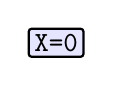
\begin{tikzpicture}[baseline=(a.base)]\node[draw=black,line width=0.8pt,fill=blue!10,rectangle,rounded corners=1pt,inner sep=2pt] (a) {\texttt{X=0}};\end{tikzpicture} $\to$ 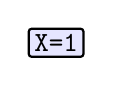
\begin{tikzpicture}[baseline=(b.base)]\node[draw=black,line width=0.8pt,fill=blue!10,rectangle,rounded corners=1pt,inner sep=2pt] (b) {\texttt{X=1}};\end{tikzpicture}} node[below] {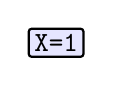
\begin{tikzpicture}[baseline=(c.base)]\node[draw=black,line width=0.8pt,fill=blue!10,rectangle,rounded corners=1pt,inner sep=2pt] (c) {\texttt{X=1}};\end{tikzpicture} $\to$ 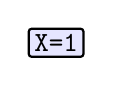
\begin{tikzpicture}[baseline=(d.base)]\node[draw=black,line width=0.8pt,fill=blue!10,rectangle,rounded corners=1pt,inner sep=2pt] (d) {\texttt{X=1}};\end{tikzpicture}} (state2);
	  
	  % From state2 to final states
	  \draw[->] ([yshift=4pt]state2.east) to[out=50,in=180] node[above, sloped] {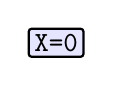
\begin{tikzpicture}[baseline=(a.base)]\node[draw=black,line width=0.8pt,fill=blue!10,rectangle,rounded corners=1pt,inner sep=2pt] (a) {\texttt{X=0}};\end{tikzpicture} $\to$ 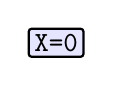
\begin{tikzpicture}[baseline=(b.base)]\node[draw=black,line width=0.8pt,fill=blue!10,rectangle,rounded corners=1pt,inner sep=2pt] (b) {\texttt{X=0}};\end{tikzpicture}} (state3.west);
	  \draw[->] ([yshift=-16pt]state2.east) to[out=-50,in=180] node[below, sloped] {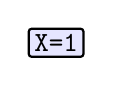
\begin{tikzpicture}[baseline=(a.base)]\node[draw=black,line width=0.8pt,fill=blue!10,rectangle,rounded corners=1pt,inner sep=2pt] (a) {\texttt{X=1}};\end{tikzpicture} $\to$ 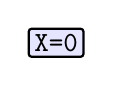
\begin{tikzpicture}[baseline=(b.base)]\node[draw=black,line width=0.8pt,fill=blue!10,rectangle,rounded corners=1pt,inner sep=2pt] (b) {\texttt{X=0}};\end{tikzpicture}} (state4.west);
	  
	  % To responses
	  \draw[->] (state3) -- (resp0);
	  \draw[->] (state4) -- (resp1);
	  
	\end{tikzpicture}
	
	\caption{Network system for the program in Listing~\ref{lst:MotivatingExample2NonSer}. Local states consist of local variable assignments and a remaining program text. Edges in the NS are labeled with their corresponding global state transition(s). Requests and responses are diamonds. For the explicit schemes of \(\delta\), \(req\), and \(resp\) see Appendix~\ref{appendix:delta-req-resp-examples}.}
\label{fig:code2ExampleNS}
\end{figure}


